\section{$tt\bar{h}$ 分析结果}\label{sec:ttH_results}
\subsection{\ltwotau 结果}
首先忽略归一化或者形状影响低于0.5\%的系统误差,最终考虑的系统误差如图~\ref{Fig:1l2tau.pruning}所列。图~\ref{Fig:1l2tau.nuispar}展示冗余参数拟合前和拟合后对信号强度的影响($\theta_{fit}-\theta_{0}/\Delta\theta$);图~\ref{Fig:1l2tau.asimov}给出拟合前和拟合后BDT的分布。最终给出的期望信号强度为:$$\mu_{ttH}=1.00^{+0.88}_{-0.75}(stat)^{+0.85}_{-0.69}(syst)=1.00^{+1.22}_{-1.02}(total)$$,对应0.98个标准偏差。系统误差间的相关性和系统误差影响排序如图~\ref{Fig:1l2tau.impacts}所示,最大的误差是假$\tau_{\text{had}}$的统计误差。

\begin{figure}[htbp]
\centering
\begin{center}
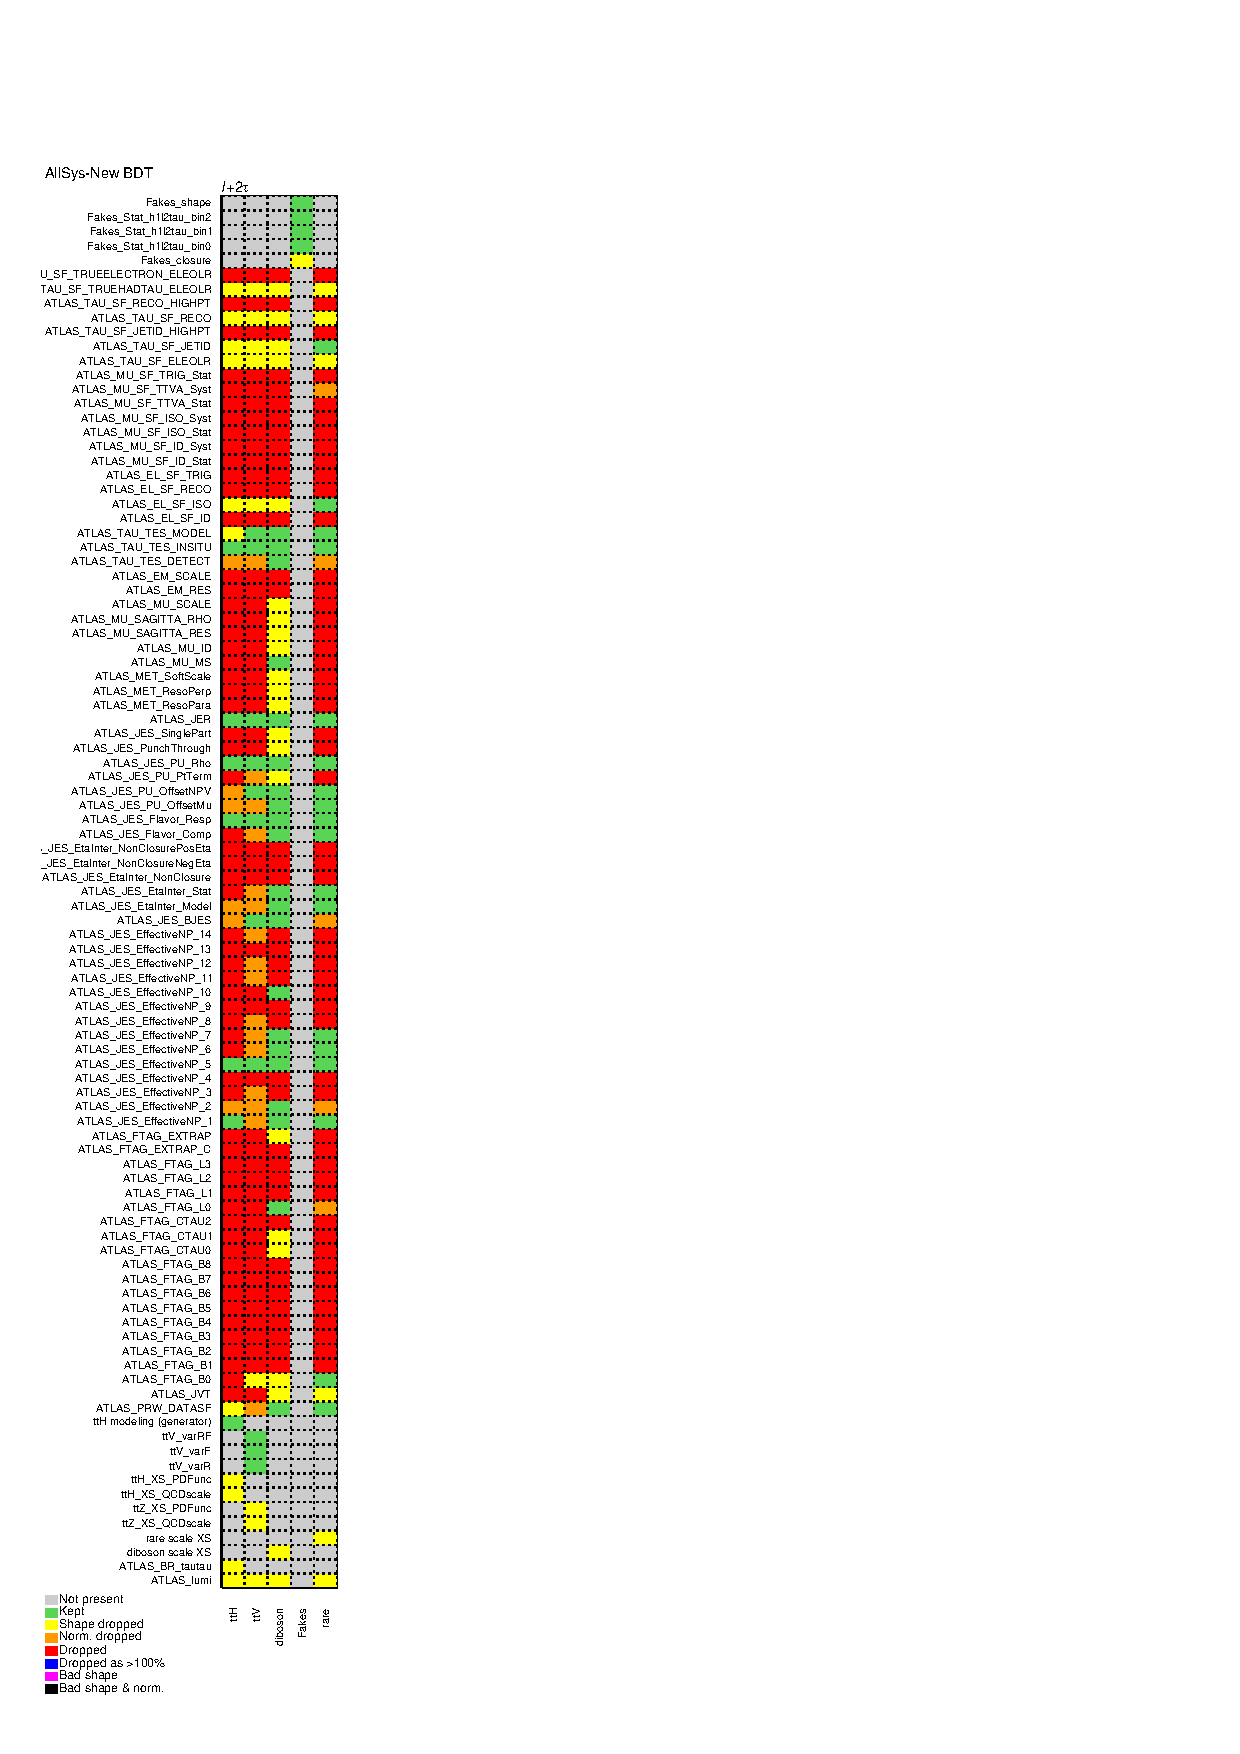
\includegraphics[width=0.35\textwidth, height=0.8\textheight]{fig/OneLepTwoTaus/Pruning.pdf}
\end{center}
\caption{\ltwotau 拟合中考虑的系统误差总结,绿色表示存在(同时影响形状和大小),黄色表示只影响大小。}
%\caption{The systematics used in the \texttt{fitter}.}
\label{Fig:1l2tau.pruning}
\end{figure}

\begin{figure}[htbp]
\centering
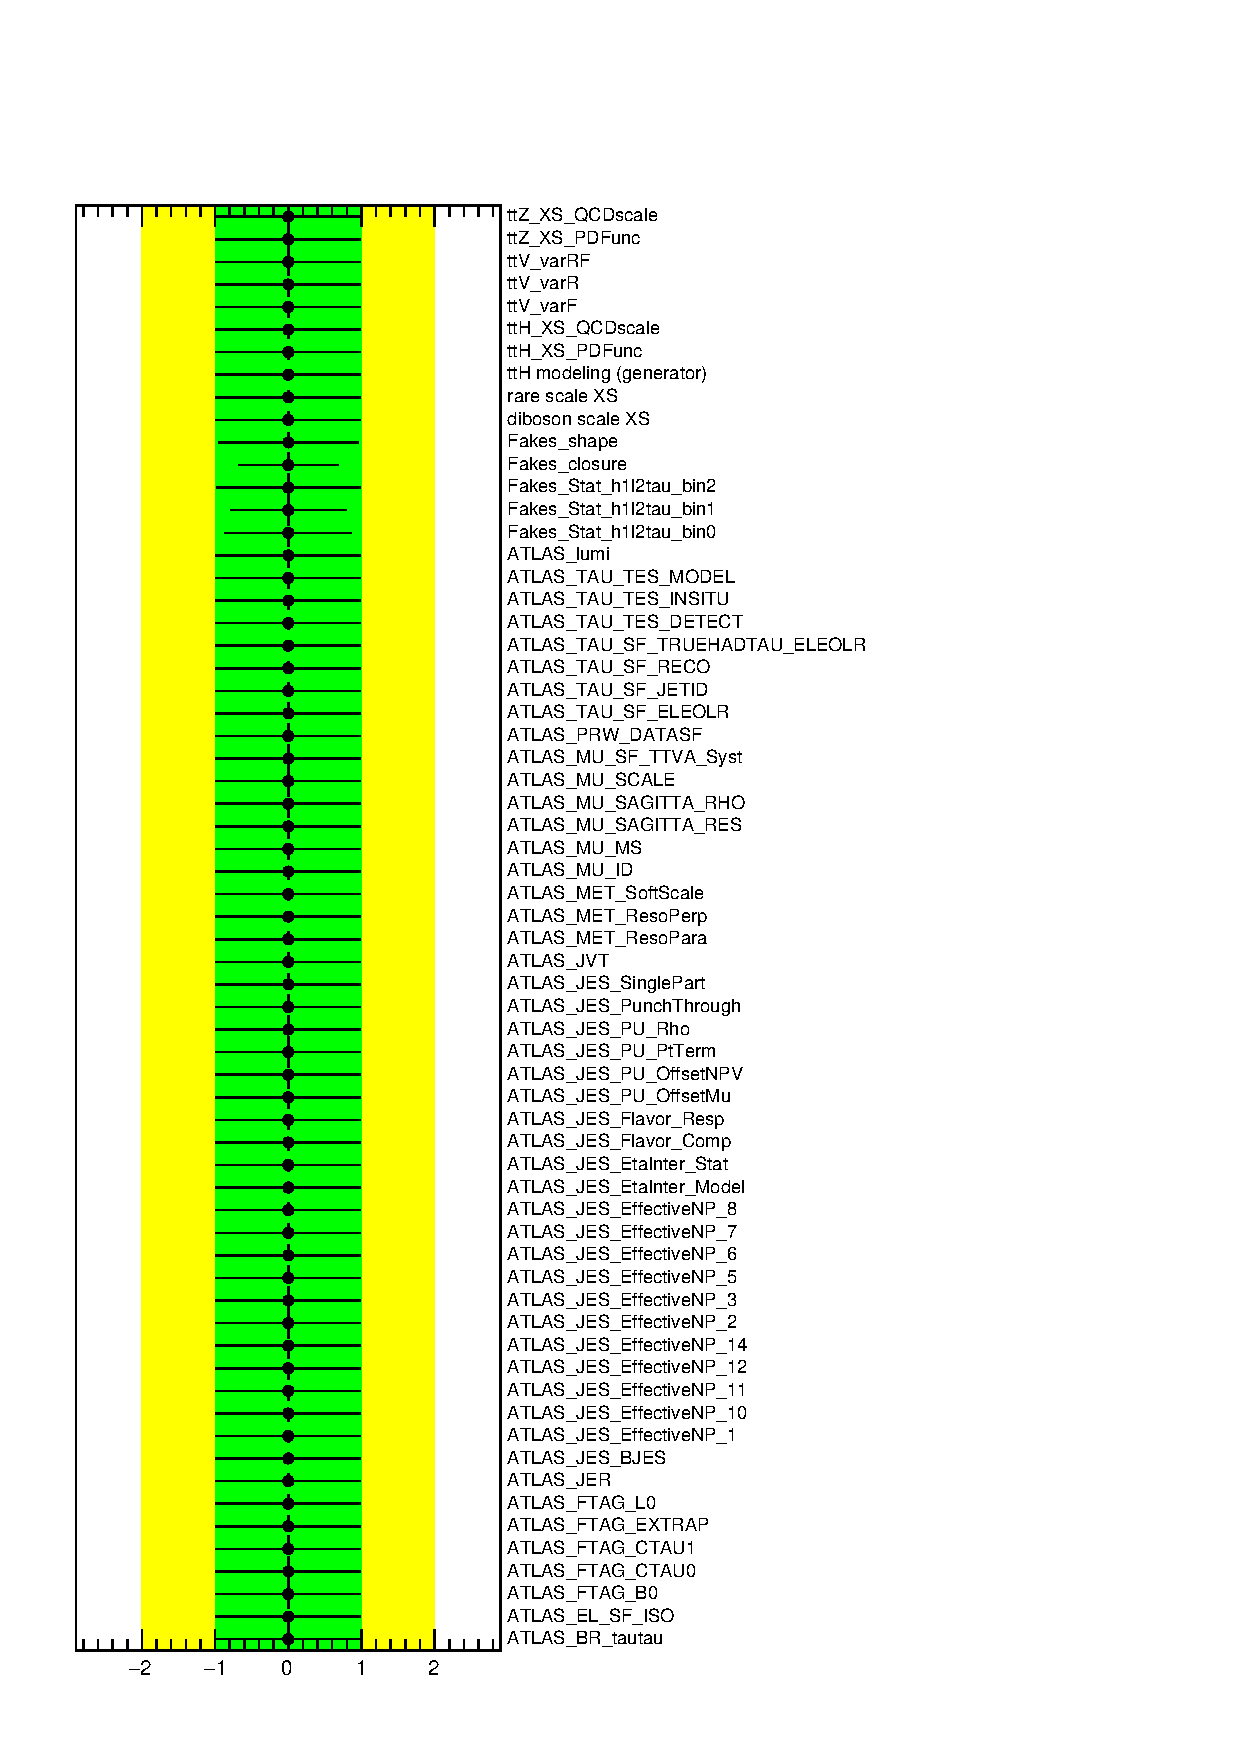
\includegraphics[width=0.7\textwidth, keepaspectratio]{fig/OneLepTwoTaus/NuisPar.pdf}
\caption{\ltwotau 系统误差pull。}
%\caption{The pull plot for systematics.}
\label{Fig:1l2tau.nuispar}
\end{figure}

\begin{figure}[htbp]
\centering
\begin{center}
  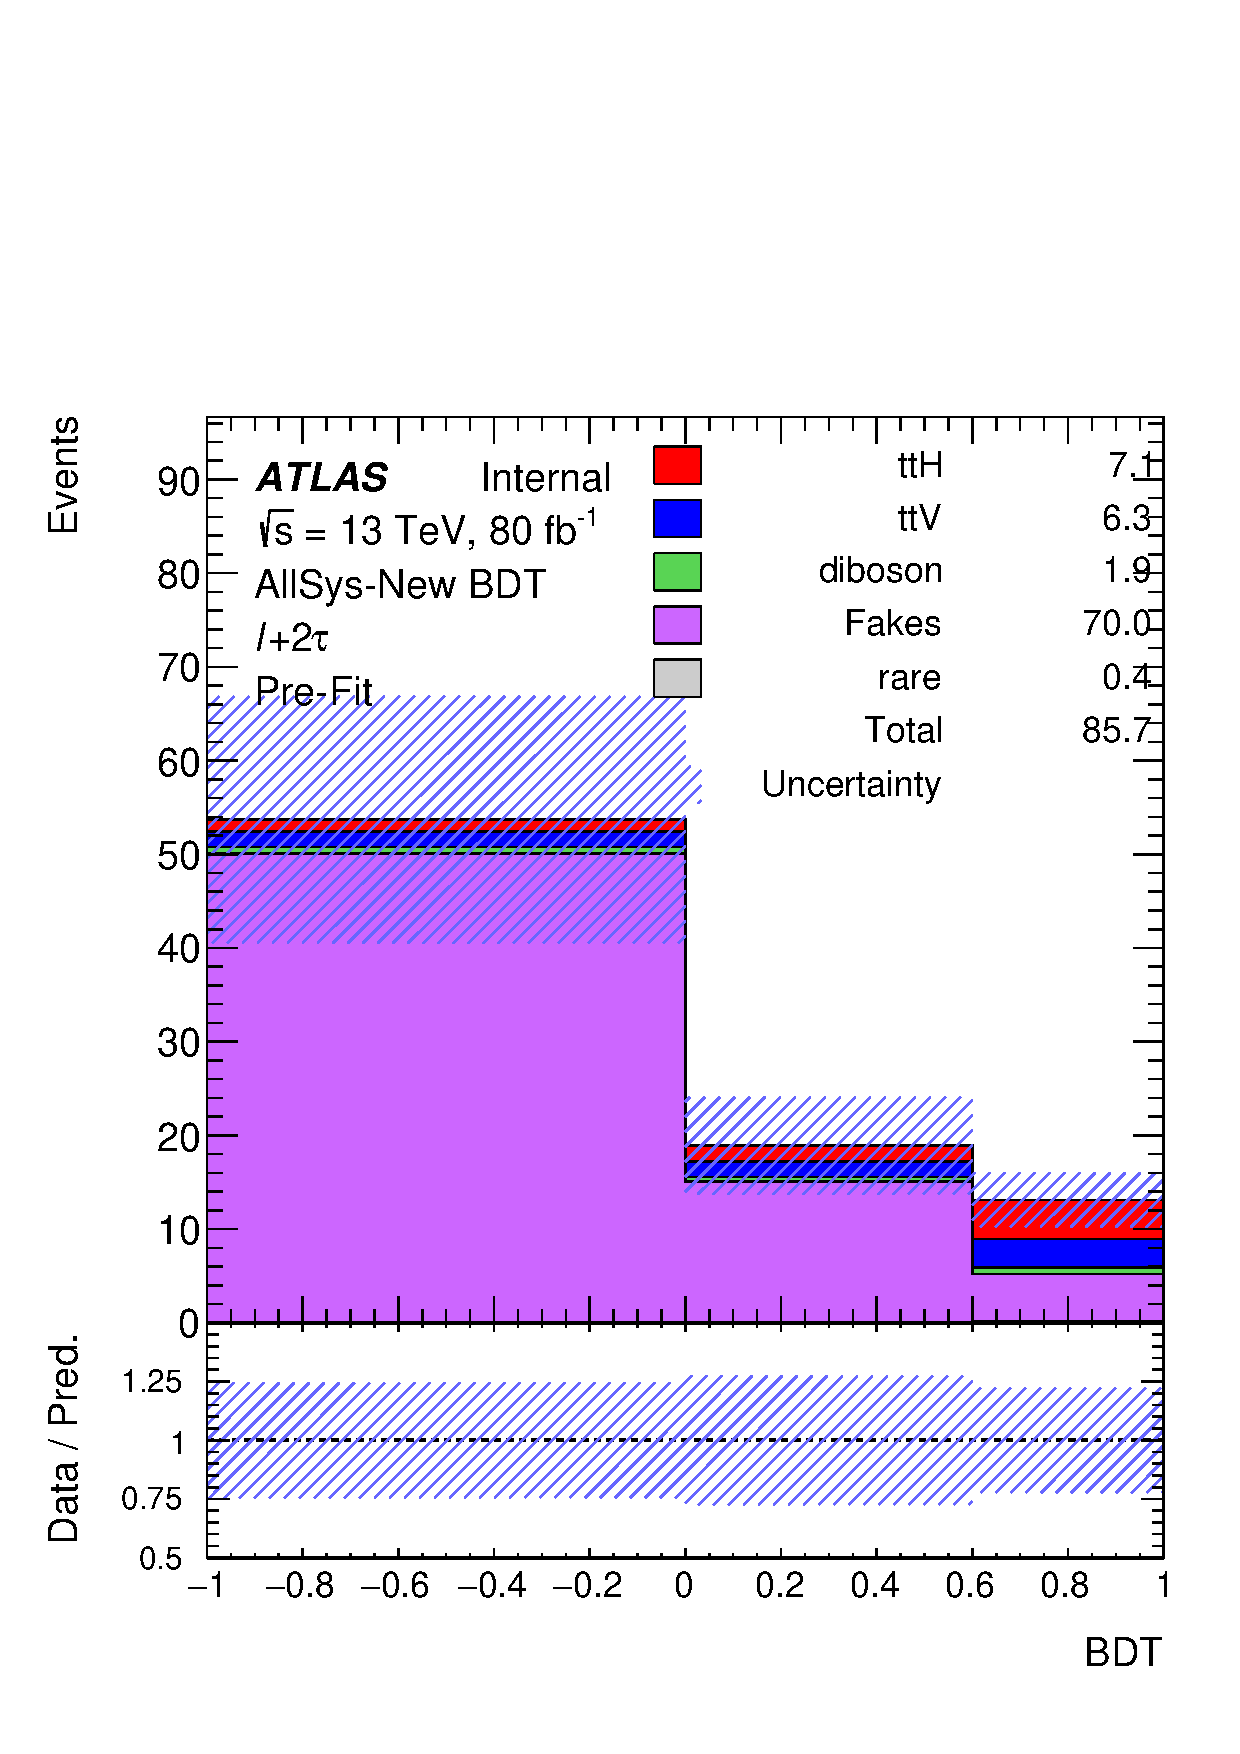
\includegraphics[width=0.45\textwidth, keepaspectratio]{fig/OneLepTwoTaus/h1l2tau.pdf}
  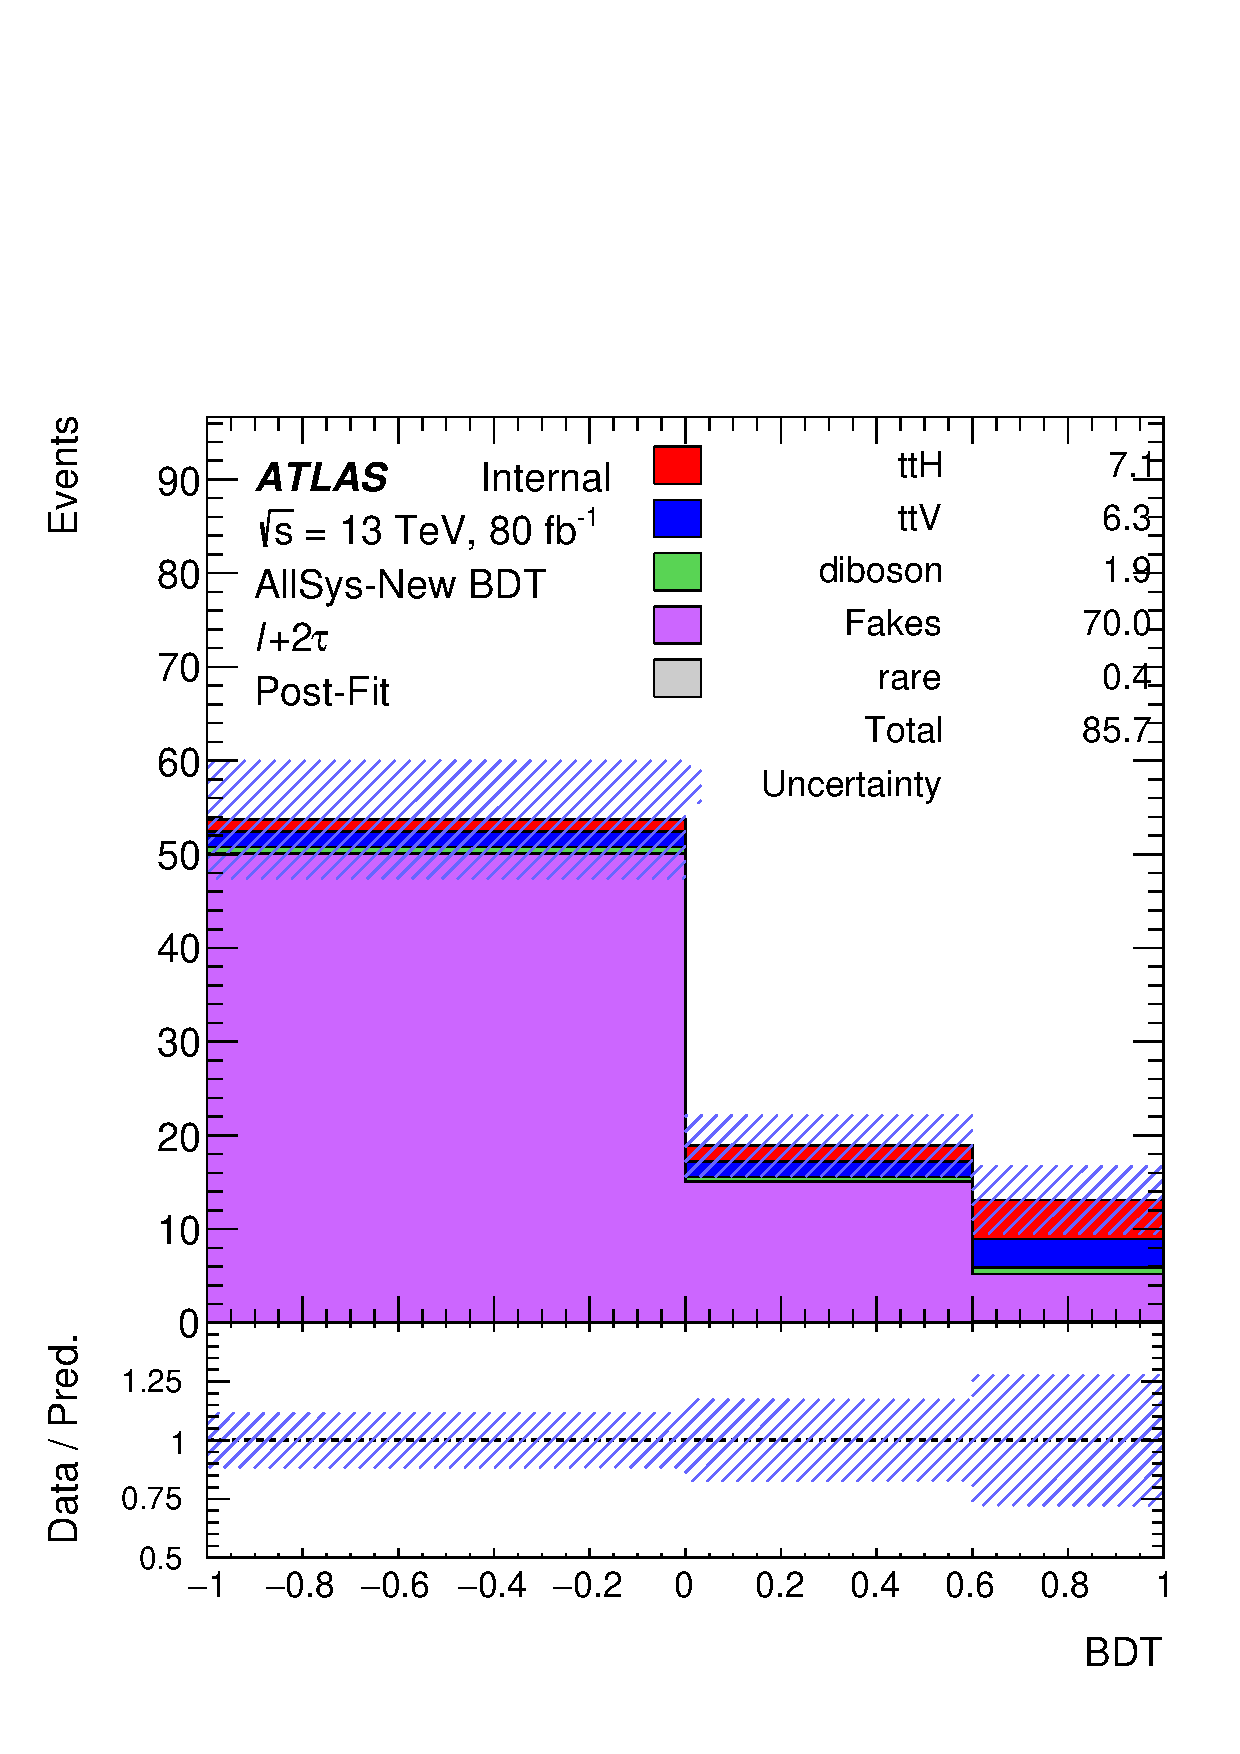
\includegraphics[width=0.45\textwidth, keepaspectratio]{fig/OneLepTwoTaus/h1l2tau_postFit.pdf}
\end{center}
\caption{Asimov数据pre-fit与post-fit结果。}
%\caption{The BDT Asimov data are shown in pre-fit (left) and post-fit (right). 
%({\bf update})
%}
\label{Fig:1l2tau.asimov}
\end{figure}

\begin{figure}[htbp]
\centering
\begin{center}
  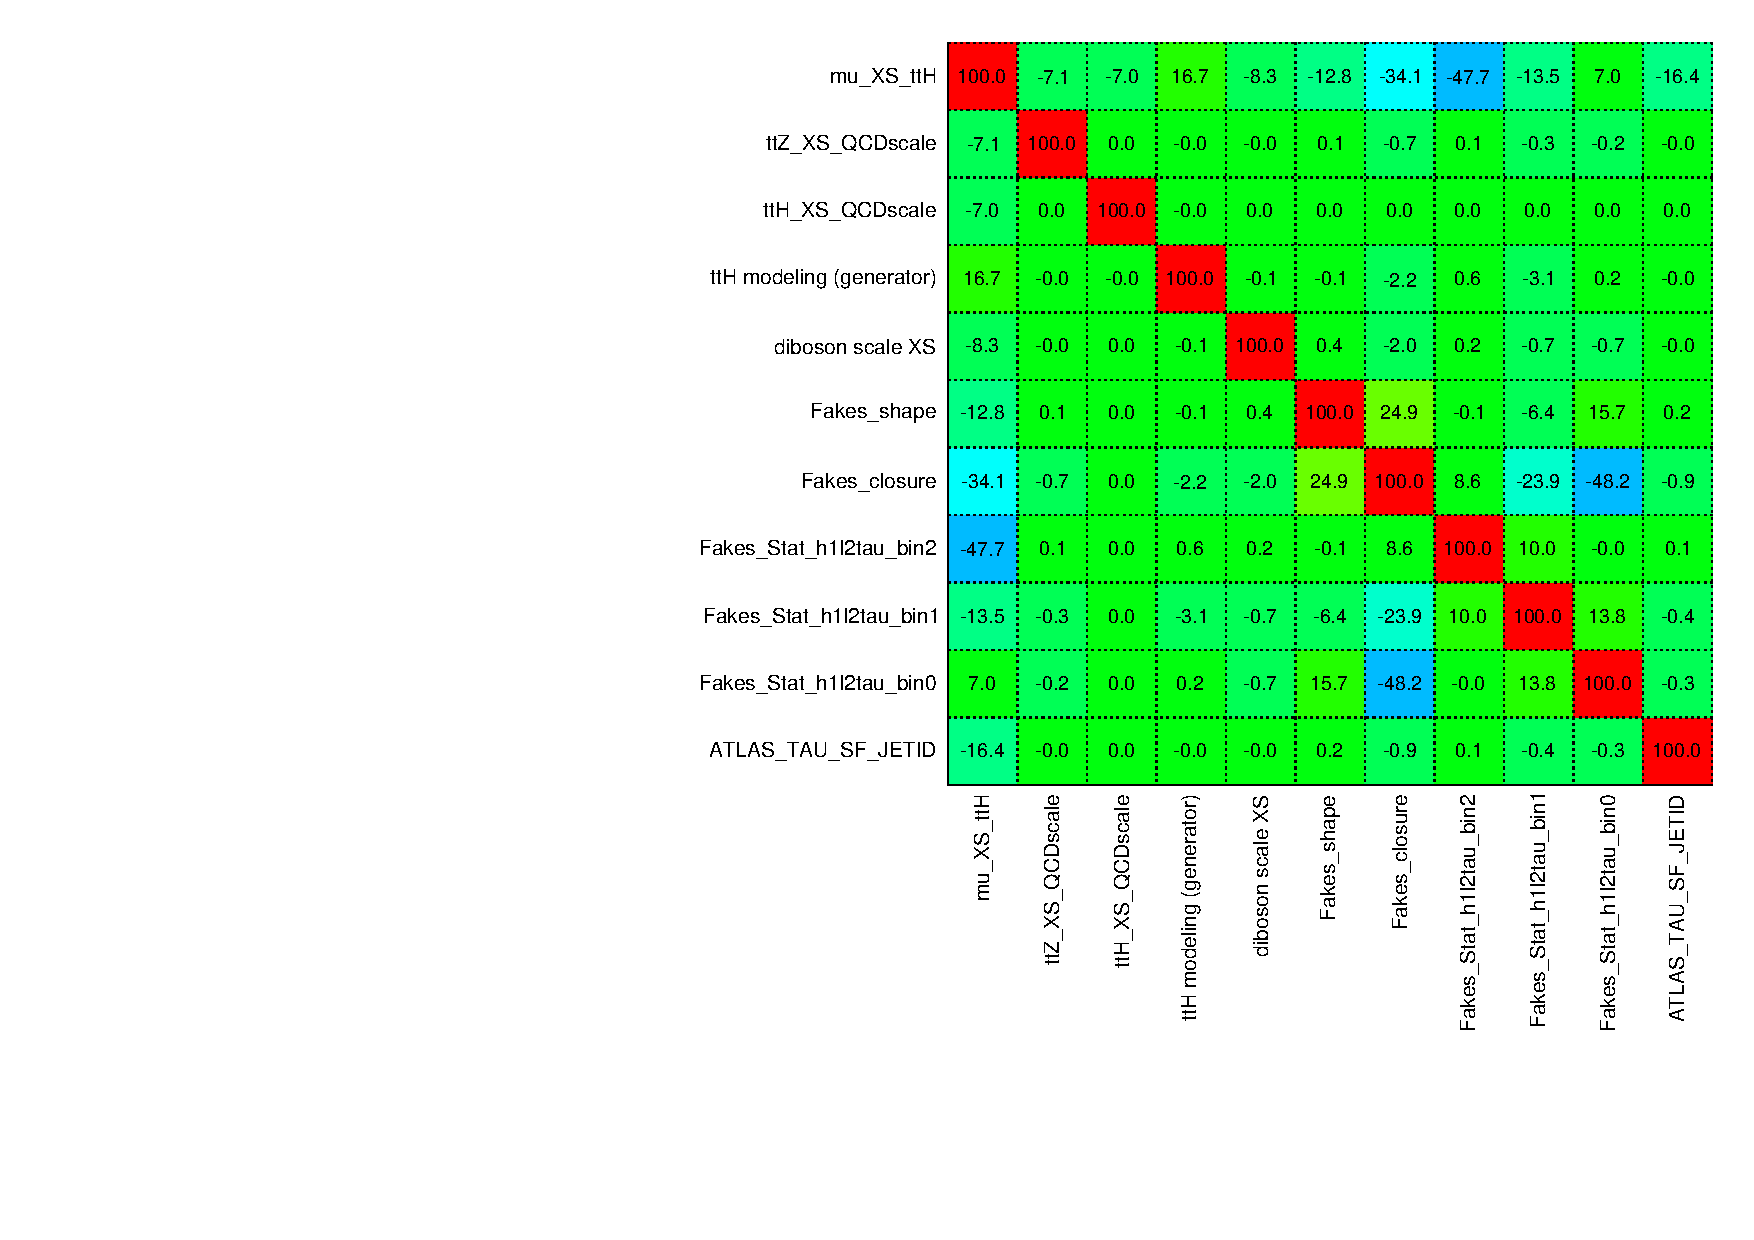
\includegraphics[width=0.45\textwidth, keepaspectratio]{fig/OneLepTwoTaus/CorrMatrix.pdf}
  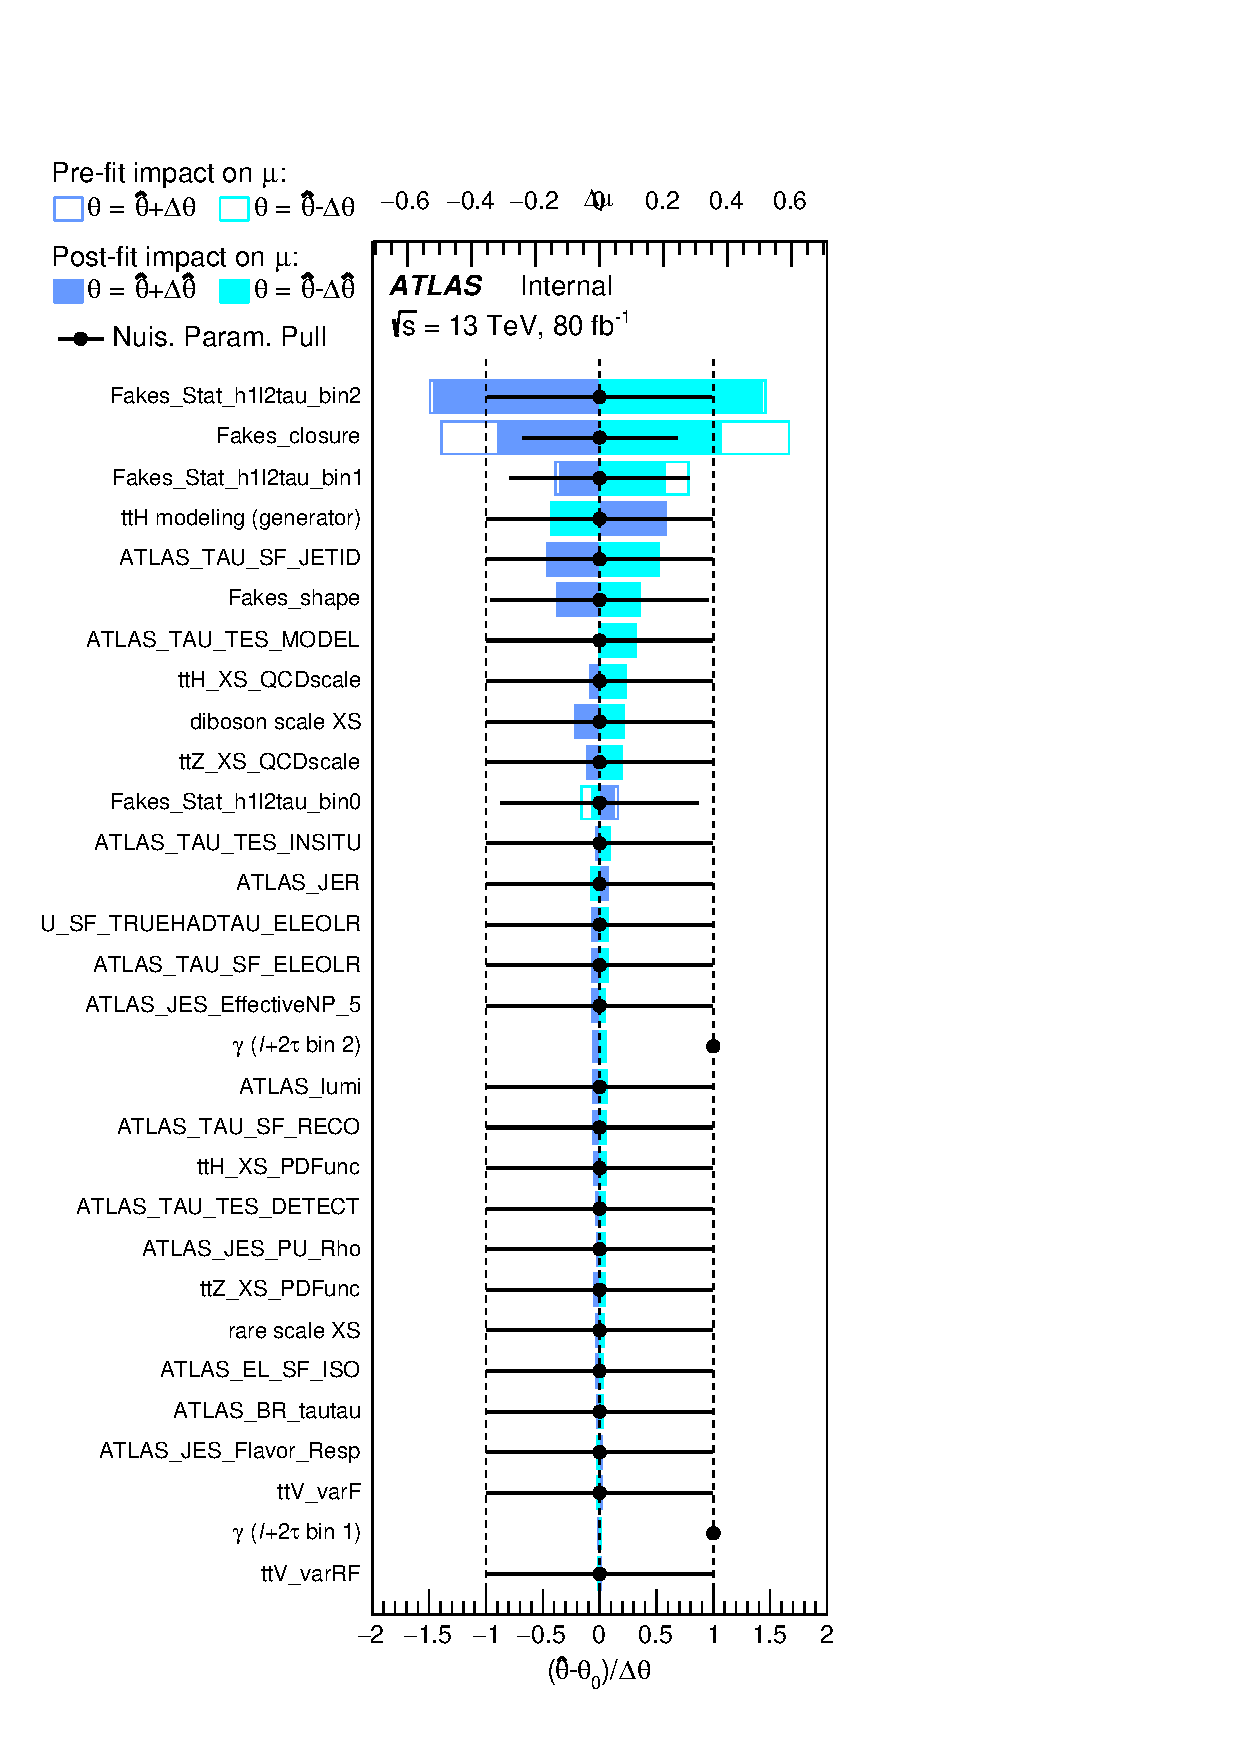
\includegraphics[width=0.5\textwidth, keepaspectratio]{fig/OneLepTwoTaus/Ranking.pdf}
\end{center}
\caption{左图:系统误差之间的关联性;右图:系统误差影响排名。}
%\caption{Left: the fitted correlation; Right: ranking of systematic based on their impacts on the signal strength measurements. 
%({\bf update})
%}
\label{Fig:1l2tau.impacts}
\end{figure}

\subsection{tthML联合统计结果}
%\textbf{Still working on unblinding approval, otherwise will put expected results only.}
与\ltwotau 分析道一样,其他分析道最终的信号强度也通过拟合构建的MVA变量得到。
$2\ell\text{SS}$总共有13个区域,包括$t\bar{t}h$信号区,以及为各种本底专门设计的区域,
分为$t\bar{t}W$, $t\bar{t}$, 来源于探测器材料反应的假轻子,光子转换的假轻子。
$3\ell$总共有7个区域,包括信号区,以及为各种本底专门设计的区域,分为$t\bar{t}W$, $t\bar{t}$, $t\bar{t}Z$, $VV$,来源于探测器材料反应的假轻子和光子转换的假轻子。
$2\ell\text{SS}$与$3\ell$均使用所谓的template fit方法去估计本底,即通过拟合得到以上本底的归一化因子。
$4\ell$根据$Z$本底的大小分为两个区域。
$2\ell\text{SS}+1\tau_{\text{had}}$和$3\ell+1\tau_{\text{had}}$均只有一个信号区。
最终拟合中各个分析道所使用的控制区域和信号区域总结在表\ref{tbl:srvr}。
\begin{table}[h]
 \centering
 \scalebox{0.8}{
 \begin{tabular}{ll}
  \hline\hline
  Channel & Selection criteria\\
  \hline \hline
  Common & $N_{\text{jets}}\ge$ 2 and $N_{b-\text{jets}} \ge 1$\\
  \hline
  \ll  & Two same-charge T* leptons, $\pt > 20$~GeV\\
       & Zero \tauhad\\
       %      & $\njets \ge 4$; $\nbjets = 1,2$\\
       & \textbf{13 categories}: enriched with \tth, \ttw, \ttbar, mat. conv, int. conv.,\\
           & split by lepton flavor, charge, jet and b-jet multiplicity \\

  \hline
  \lll & Three L light leptons with $\pt > 10$~GeV; sum of light lepton charges $\pm 1$ \\
       & Two same-charge T* leptons, $\pt > 15$ GeV\\
       & Opposite-charge L* lepton, $\pt > 10$ GeV\\
       & Zero \tauhad\\
       & $m(\ell^+\ell^-) > 12$~GeV and $|m(\ell^+\ell^-)-91.2\textrm{ GeV}| > 10$~\textrm{GeV} for all SFOC pairs\\
       & $|m(3\ell)-91.2\textrm{ GeV}| > 10$~\textrm{GeV}\\
       & \textbf{7 categories}: enriched with \tth, \ttw, \ttz, diboson, \ttbar, mat. conv, int. conv \\

  \hline
  \llll   & Four L* leptons; sum of light lepton charges 0 \\
          & $m(\ell^+\ell^-) > 12$~GeV and $|m(\ell^+\ell^-)-91.2\textrm{ GeV}| > 10$~GeV for all SFOC pairs \\
          & $m(4\ell) < 115\textrm{ GeV}$ and $m(4\ell) > 130\textrm{ GeV}$\\
          & \textbf{2 categories}: $Z$-depleted (0 SFOC pairs) and $Z$-enriched (2 or 4 SFOC pairs)\\

  \hline
  \ltwotau & One T lepton, $\pt > 27$~GeV \\
           & Two OC \tauhad \\
           & At least one tight \tauhad\\
           & $N_{\text{jets}} \ge 3$ \\

  \hline
  \lltau  & \ll selection, except: One \tauhad\\
  \hline
  \llltau & \lll selection, except: \\
          & One \tauhad, of opposite charge to the total charge of the light leptons \\
          & Two T same-charge leptons. $\pt > 10$ GeV\\
  \hline\hline
 \end{tabular}}
 %\caption{Offline selection criteria applied to the channels. Same-flavour, opposite-charge lepton pairs are referred to as SFOC pairs. The common selection criteria for all channels is listed in the first line under the title ``Common''.}
 \caption{tthML各个分析道拟合所涉及到的信号区域控制区。L指代通过基本筛选条件,加‘*’表示额外的孤立化条件,SFOC指代相同味道,相反电荷轻子对。}
\label{tbl:srvr}
\end{table}

图\ref{fig:SignalPlots_postfit}展示各个分析道利用Asimov数据拟合之后的信号与本底分布。表\ref{tab:expsig_tthML}给出各个分析道的期望信号强度与联合统计结果,
并且分别给出了含\tauhad 与不含\tauhad 类的联合统计结果,在80 fb$^{-1}$积分亮度下仅通过多轻子道可期望达到3$\sigma$,其中\ll 与\lll 贡献最大。
相应的信号强度为0.99$^{0.37}_{-0.31}$,如图\ref{fig:tthML_combined_strength}左侧所示,并且给出了各种假本底的归一化因子拟合值,图右侧为NP对应拟合结果的排序,
最大的系统误差为\tth 的scale理论误差,其次是\ttw 截面,喷注能量刻度,\ttz 的scale理论误差及pileup,$\gamma(\ell+2\tau)$为\ltwotau 的fakes统计误差,
因为其直接使用SS data估计,误差大小由数据量决定。
\begin{figure}[!htbp]
\centering
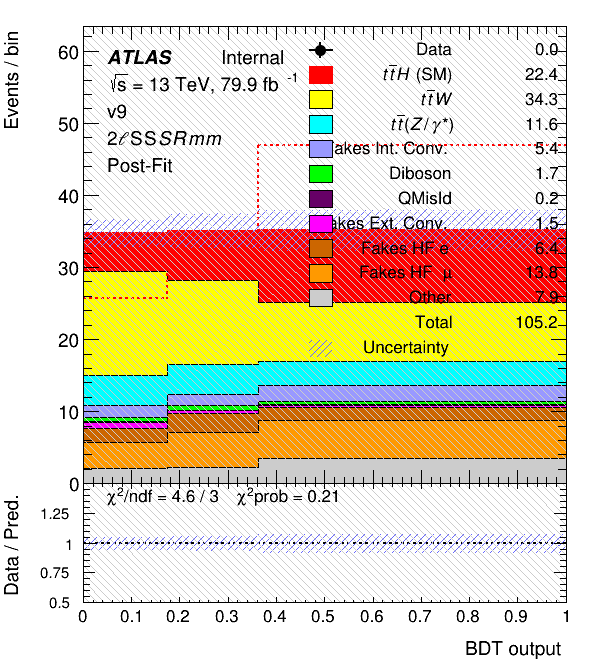
\includegraphics[width=0.31\textwidth]{plots_postfit/l20tau_SR_mm_postFit.png}
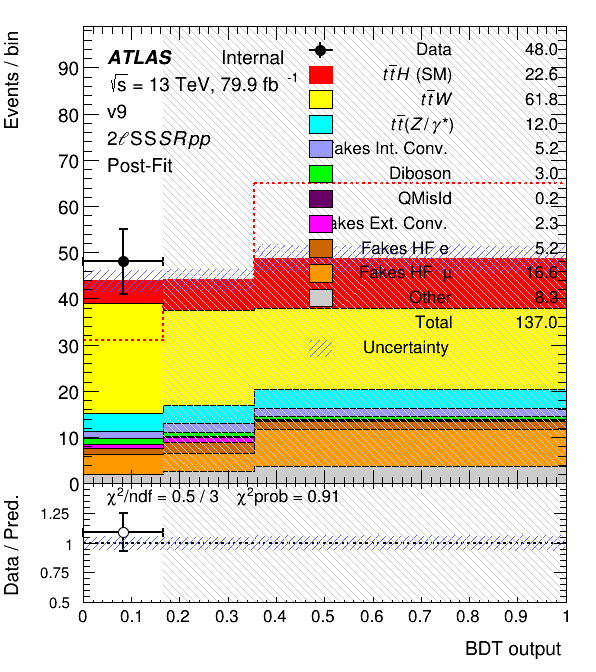
\includegraphics[width=0.31\textwidth]{plots_postfit/l20tau_SR_pp_postFit.png}
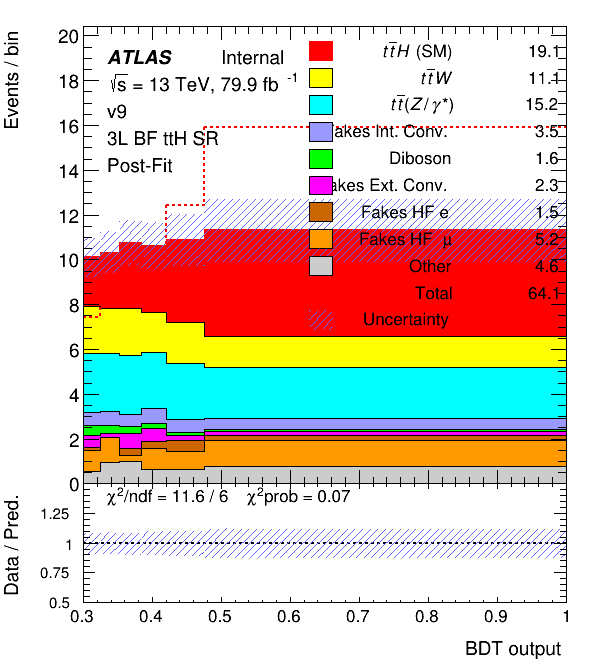
\includegraphics[width=0.31\textwidth]{plots_postfit/l30tau_ttH_postFit.png}
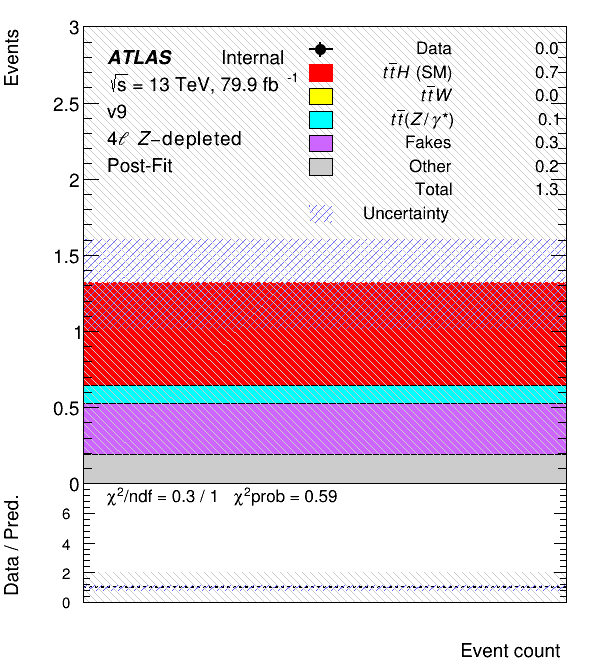
\includegraphics[width=0.31\textwidth]{plots_postfit/l4_depZ_postFit.png}
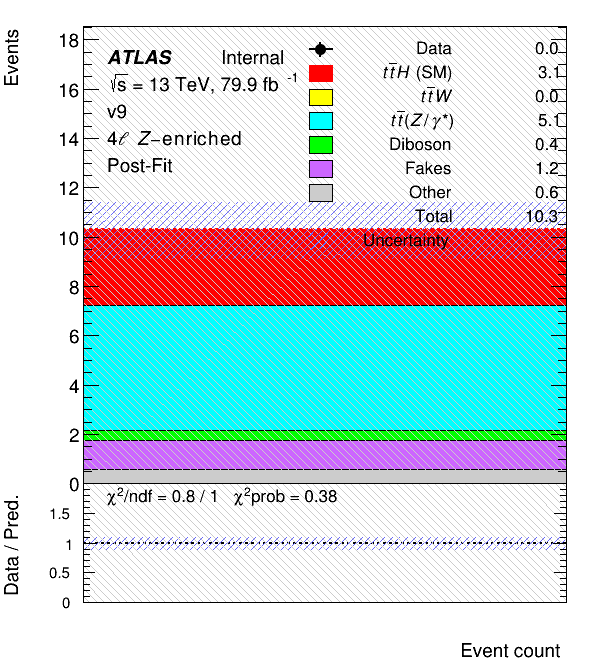
\includegraphics[width=0.31\textwidth]{plots_postfit/l4_enrZ_postFit.png}
%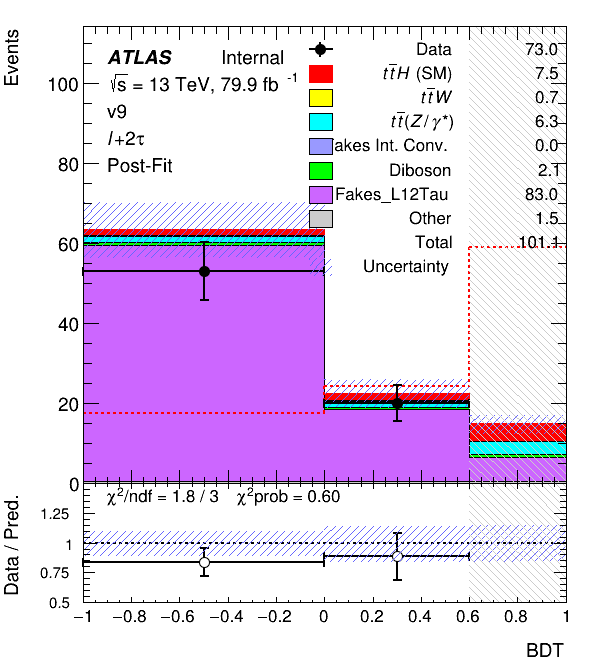
\includegraphics[width=0.31\textwidth]{plots_postfit/L12Tau_postFit.png}
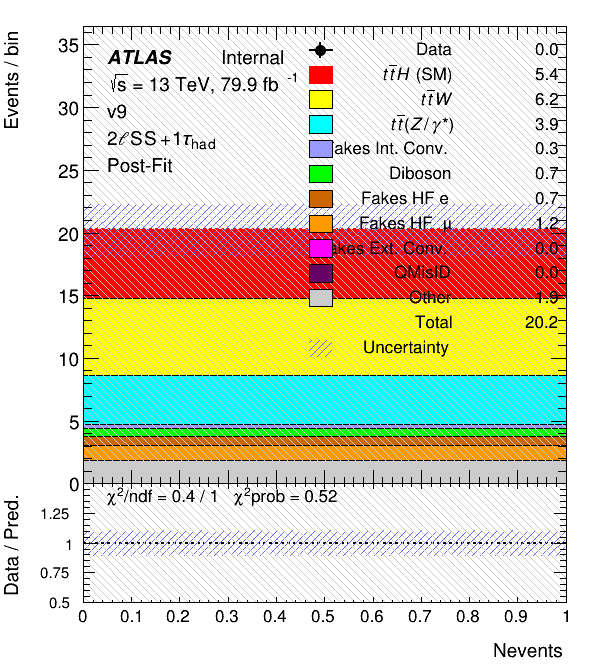
\includegraphics[width=0.31\textwidth]{plots_postfit/L2SS1Tau_postFit.png}
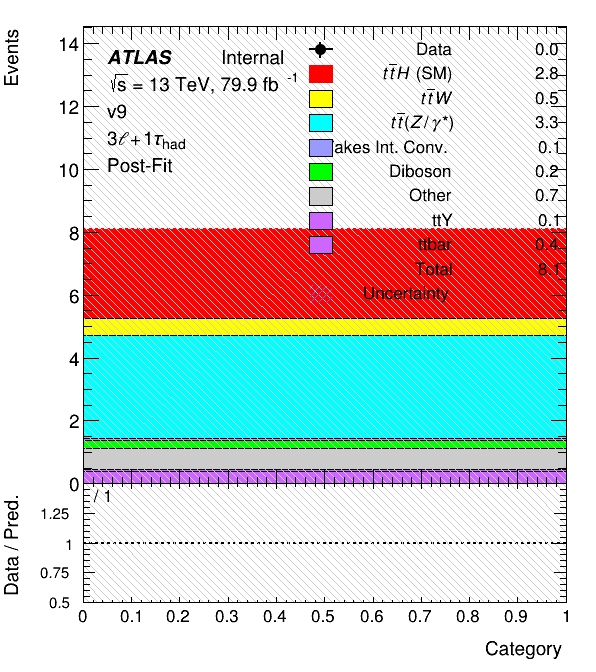
\includegraphics[width=0.31\textwidth]{plots_postfit/L31Tau_postFit.png}
 % \caption{The distributions in the signal regions after the fit, showing data (points with error bars), in the unblinded bins (S/B $< 15$\%), and expected contributions (histograms) in the \ll channel (BDT$_{\ttV}$: -- top left, ++ top middle), in the \lll channel (BDT$_{\ttH}$: top right), in the \llll channel (Z-depleted: middle left; Z-enriched: middle middle), in the \ltwotau (BDT$_{\ttbar}$: middle right), in the \lltau (bottom left) and \llltau (bottom right) channels. The size of the combined statistical and systematic uncertainty on the sum of the signal and fitted background is indicated by the blue hatched band. \label{fig:SignalPlots_postfit}}
\caption{Asimov拟合之后的信号区分布,数据只在S/B $< 15$\% bin展示。}
 \label{fig:SignalPlots_postfit}
\end{figure}

\begin{table}[htbp]
\centering
\begin{tabular}{lc}
\hline\hline
Channels.       &  {Expected significance [$\sigma$]: stat.+syst. (stat.)} \\
\hline
\ll        & 2.16 (2.56) \\
\lll       & 2.59 (2.89) \\
\llll      & 1.23 (1.27) \\
\hline
Combined Non-Tau    &   3.14 (3.70) \\
\hline
\ltwotau        &   0.96 (1.07) \\
\llltau         &   1.09 (1.13) \\
\lltau          &   1.22 (1.36) \\
\hline
Combined Tau    &   1.82 (2.07) \\
\hline
Combined &3.39 (4.12) \\
\hline \hline
\end{tabular}
%\caption{\label{tab:expsig_tau0tau}  Expected significance of the individual non-tau channels (\ll, \lll, and \llll) and its combination, from a fit with full statistical and systematic uncertainties included, as well as statistical only.}
\caption{tthML各个分析道的期望信号显著性与联合统计结果。}
\label{tab:expsig_tthML}
\end{table}

\begin{figure}[htbp]
\begin{center}
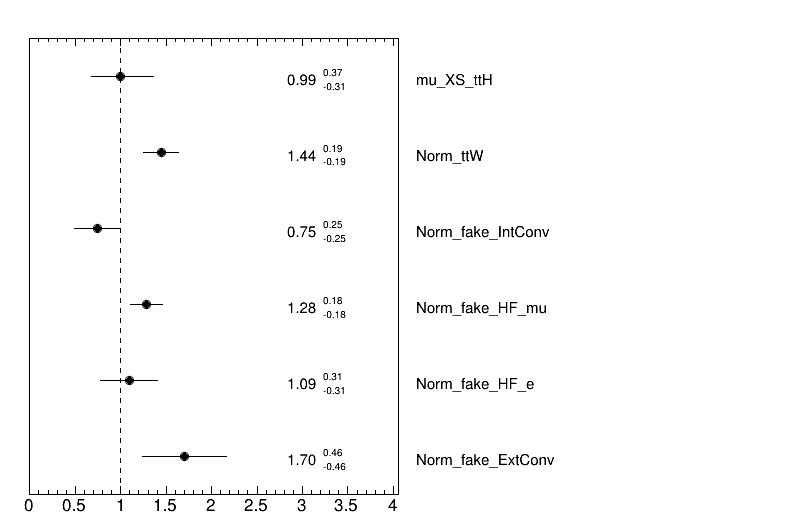
\includegraphics[width=0.4\textwidth]{OneMuFit/NormFactors.png}
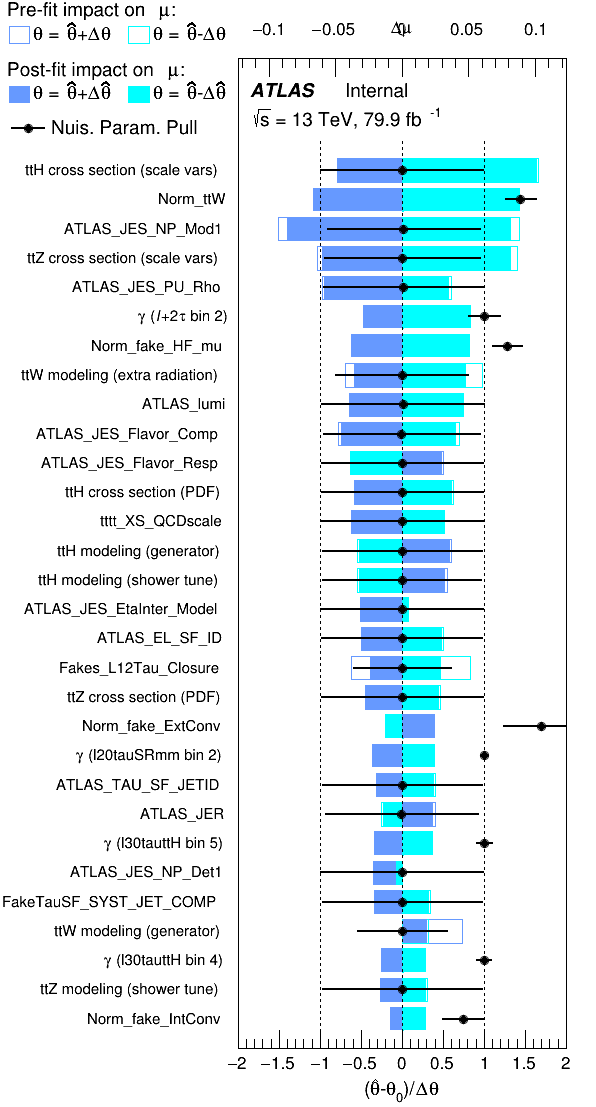
\includegraphics[width=0.5\textwidth]{OneMuFit/Ranking.png}
\end{center}
%\caption{Composition of the events for each region in the template fit.[to be updated with full syst.] \label{fig:combo} }
\caption{左:信号强度与各本底归一化Asimov拟合值;右:NP排序。}
\label{fig:tthML_combined_strength}
\end{figure}